\pdfsuppresswarningpagegroup=1

\documentclass[11pt]{article}

\usepackage{pdfpages}
\usepackage[top=1in,bottom=1in,left=1in,right=1in]{geometry} 

\renewcommand{\labelenumii}{\theenumii}			% Set first level enumerate items to use arabic numerals (1,2,3,4,etc.)
\renewcommand{\theenumii}{\arabic{enumii}.}		% Set second level enumerate items to use the same as first level with following .

\begin{document}
	\title{ \vspace{-1in}The Leftovers \\
			\Large{Use Cases} }

	\author{	Nicholas Chiapputo, Khaemon Edwards, Caleb Halter, \\
				Jacob Robbins, Ryan Vanek, Saidat Babatunde, \\
				Ephraim Emilimor, Jordan Simmons
	}

	\maketitle

	\begin{enumerate}
		\item \textbf{Name:} 				Customer Places Order

			\textbf{Participating Actors:} 	Customer | Kitchen

			\textbf{Entry Condition:} 		Customer has placed one or more items in the order

			\textbf{Exit Condition:} 		Order has been sent to the kitchen

			\textbf{Event Flow:}
			\begin{enumerate}
				\setlength{\leftskip}{1cm}
				\item Customer selects items for order.
				\item If current local time is 11:30pm or later, no items are able to be added to an order.
				\item Customer edits items as desired.
				\item Customer reviews order.
				\item Customer confirms order.
				\item System updates the inventory with respect to the items in the order. 
				\item Order is sent to the kitchen.\\
			\end{enumerate}

		\item \textbf{Name:} 				Play a Free Game

			\textbf{Participating Actors:} 	Customer

			\textbf{Entry Condition:} 		Customer is at system main menu

			\textbf{Exit Condition:} 		Customer has played a free game and has exited the game screen 

			\textbf{Event Flow:}
			\begin{enumerate}
				\setlength{\leftskip}{1cm}
				\item Customer clicks “Game” button.
				\item System switches to screen with a list of games.
				\item System temporarily suspends options for placing an order, asking for help or requesting a refill.
				\item Customer chooses a game to play.
				\item Customer plays game.
				\item Customer exits the game
				\item System resumes and exits the game screen, allowing the customer to place an order, ask for help, or request a refill. \\
			\end{enumerate}

		\item \textbf{Name:} 				Customer Calls Server For Help

			\textbf{Participating Actors:} 	Customer | Server

			\textbf{Entry Condition:} 		Customer is not in kid's mode

			\textbf{Exit Condition:} 		Server has received help notification

			\textbf{Event Flow:}
			\begin{enumerate}
				\setlength{\leftskip}{1cm}
				\item Customer selects option to call for help.
				\item Server receives notification for help from customer.\\
			\end{enumerate}

		\item \textbf{Name:} 				Send Request for Refill

			\textbf{Participating Actors:} 	Customer | Server

			\textbf{Entry Condition:} 		Customer is not in kid's mode

			\textbf{Exit Condition:} 		Server has received refill request

			\textbf{Event Flow:}
			\begin{enumerate}
				\setlength{\leftskip}{1cm}
				\item Customer selects optio to request a refill
				\item Server receives refill request notification\\
			\end{enumerate}

		\item \textbf{Name:} 				Customer Pays for Order(s)

			\textbf{Participating Actors:} 	Customer

			\textbf{Entry Condition:} 		Customer has placed one or more orders

			\textbf{Exit Condition:} 		Customer receives receipt

			\textbf{Event Flow:}
			\begin{enumerate}
				\setlength{\leftskip}{1cm}
				\item Customer selects “Pay Now” button.
				\item Customer splits order by selecting which menu items they wish to pay for.
				\item System displays the amount due including tax.
				\item Customer applies applicable coupons to order.
				\item Customer adds desired tip amount for server.
				\item Customer adds special note to server if desired.
				\item Customer pays the amount due.
				\item Customer selects print or email receipt option after the transaction has been processed.\\
			\end{enumerate}

		\newpage

		\item \textbf{Name:} 				Kid's Discount

			\textbf{Participating Actors:} 	Customer

			\textbf{Entry Condition:} 		It is Monday between the hours of 4:00pm and 11:59pm | At least one entr\`e has beeen ordered

			\textbf{Exit Condition:} 		Customer has received a free kid's meal

			\textbf{Event Flow:}
			\begin{enumerate}
				\setlength{\leftskip}{1cm}
				\item Customer adds kid's meal to order.
				\item Kid's meal price is reduced to \$0.00 for each entree that has been ordered.\\
			\end{enumerate}

		\item \textbf{Name:} 				Win Dessert

			\textbf{Participating Actors:} 	Customer

			\textbf{Entry Condition:} 		Customer has paid all orders in full

			\textbf{Exit Condition:} 		Customer has finished playing dessert game

			\textbf{Event Flow:}
			\begin{enumerate}
				\setlength{\leftskip}{1cm}
				\item Customer is given option to play game for a chance to win a free dessert.
				\item CUstomer wins a coupon for a free dessert with a 1 in 5 chance.\\
			\end{enumerate}

		\item \textbf{Name:} 				Server Checks Table Status

			\textbf{Participating Actors:} 	Server

			\textbf{Entry Condition:} 		Server is on the main menu

			\textbf{Exit Condition:} 		Server is given table status

			\textbf{Event Flow:}
			\begin{enumerate}
				\setlength{\leftskip}{1cm}
				\item Server selects “Tables” from the main menu.
				\item Tables are displayed under the headings “Ordered”, “Eating”, and “Paid” with appropriate table numbers.\\
			\end{enumerate}

		\item \textbf{Name:} 				Server Logs Into System

			\textbf{Participating Actors:} 	Server

			\textbf{Entry Condition:} 		Server's device is not logged in

			\textbf{Exit Condition:} 		Server is logged in to device

			\textbf{Event Flow:}
			\begin{enumerate}
				\setlength{\leftskip}{1cm}
				\item Server enters credentials on login screen.
				\item Server selects ``Clock In'' button.
				\item If credentials are incorrect, the server is returned to the login screen.
				\item If credentials are correct, server is logged in to the system.\\
			\end{enumerate}

		\item \textbf{Name:} 				Server Logs Out of System

			\textbf{Participating Actors:} 	

			\textbf{Entry Condition:} 		

			\textbf{Exit Condition:} 		

			\textbf{Event Flow:}
			\begin{enumerate}
				\setlength{\leftskip}{1cm}
				\item Server selects the ``Clock Out'' option on the menu.
				\item Server is automatically clocked out and returned to the login screen.\\
			\end{enumerate}

		\item \textbf{Name:} 				Server Places Order

			\textbf{Participating Actors:} 	Server | Customer | Kitchen

			\textbf{Entry Condition:} 		Server is on table status screen

			\textbf{Exit Condition:} 		Order has been sent to the kitchen

			\textbf{Event Flow:}
			\begin{enumerate}
				\setlength{\leftskip}{1cm}
				\item Server selects appropriate table number.
				\item Server selects ``View Order'' option for the table.
				\item Server adds customer’s desired items with any desired modifications.
				\item Server confirms order.
				\item Order is sent to the kitchen.\\
			\end{enumerate}

		\item \textbf{Name:} 				Server Processes Payment

			\textbf{Participating Actors:} 	Server | Customer

			\textbf{Entry Condition:} 		Customer has placed order and server is on table status screen

			\textbf{Exit Condition:} 		Payment has been processed

			\textbf{Event Flow:}
			\begin{enumerate}
				\setlength{\leftskip}{1cm}
				\item Server selects appropriate table number
				\item Server selects ``View Bill'' option for the table.
				\item Server adds coupon codes as necessary.
				\item Server splits the bill as necessary.
				\item Server selects ``Pay'' option and processes the payment with desired payment method.\\
			\end{enumerate}

		\newpage

		\item \textbf{Name:} 				Server Comps Order

			\textbf{Participating Actors:} 	Server | Customer

			\textbf{Entry Condition:} 		Customer has placed order and server is on table status screen

			\textbf{Exit Condition:} 		Order has been comped

			\textbf{Event Flow:}
			\begin{enumerate}
				\setlength{\leftskip}{1cm}
				\item Server selects appropriate table number.
				\item Server selects ``View Bill'' option for the table.
				\item Server selects ``Comp Order'' option on bill screen.
				\item Server selects items to be comped
				\item Server confirms selections and the desired items are comped\\
			\end{enumerate}

		\item \textbf{Name:} 				Server Calls Manager for Assistance

			\textbf{Participating Actors:} 	Server | Manager

			\textbf{Entry Condition:} 		Server is in front of device

			\textbf{Exit Condition:} 		Manager has received notification for help

			\textbf{Event Flow:}
			\begin{enumerate}
				\setlength{\leftskip}{1cm}
				\item Server selects ``Call Manager'' button at the top of any screen on the device.
				\item Manager receives notification that the server requires assistance.\\
			\end{enumerate}

		\item \textbf{Name:} 				Server Receives Completed Order Notifications

			\textbf{Participating Actors:} 	Server | Kitchen

			\textbf{Entry Condition:} 		Order has been sent to kitchen

			\textbf{Exit Condition:} 		Server receives completed order notification

			\textbf{Event Flow:}
			\begin{enumerate}
				\setlength{\leftskip}{1cm}
				\item Once the kitchen has completed order, they mark it as complete.
				\item Server receives notification that order has been marked as complete.\\
			\end{enumerate}

		\newpage

		\item \textbf{Name:} 				Kitchen Calls Server for Help

			\textbf{Participating Actors:} 	Kitchen | Server

			\textbf{Entry Condition:} 		Kitchen staff is on kitchen system menu

			\textbf{Exit Condition:} 		Server receives notification for help

			\textbf{Event Flow:}
			\begin{enumerate}
				\setlength{\leftskip}{1cm}
				\item Kitchen staff clicks ``Help'' button.
				\item Kitchen staff selects server to call.
				\item Kitchen staff selects ``Call Server''.
				\item Server receives help notification.\\
			\end{enumerate}

		\item \textbf{Name:} 				Kitchen Calls Manager for Help

			\textbf{Participating Actors:} 	Kitchen | Manager

			\textbf{Entry Condition:} 		Kitchen staff is on kitchen system menu

			\textbf{Exit Condition:} 		Manager receives notification for help

			\textbf{Event Flow:}
			\begin{enumerate}
				\setlength{\leftskip}{1cm}
				\item Kitchen staff clicks ``Help'' button.
				\item Kitchen staff selects ``Call Manager''.
				\item Manager receives help notification.\\
			\end{enumerate}

		\item \textbf{Name:} 				Kitchen Marks Order as Complete

			\textbf{Participating Actors:} 	Kitchen

			\textbf{Entry Condition:} 		Kitchen staff is on kitchen system menu

			\textbf{Exit Condition:} 		Order has been marked as complete

			\textbf{Event Flow:}
			\begin{enumerate}
				\setlength{\leftskip}{1cm}
				\item Kitchen staff selects order from list.
				\item Kitchen staff selects individual meal from order.
				\item Kitchen staff marks meal as completed.
				\item Kitchen staff marks order as completed when all meals are marked complete.\\
			\end{enumerate}

		\newpage

		\item \textbf{Name:} 				Add Menu Item to Menu

			\textbf{Participating Actors:} 	Manager

			\textbf{Entry Condition:} 		Manager is at system main menu

			\textbf{Exit Condition:} 		Item has been added to menu

			\textbf{Event Flow:}
			\begin{enumerate}
				\setlength{\leftskip}{1cm}
				\item Manager clicks ``Edit Menu'' button.
				\item Manager types ``Add Item'' button.
				\item Manager enters item’s title, description, nutritional information, customization options, and allergen information in respective fields.
				\item Manager clicks ``Upload Image'' button and selects an image on his/her local disc.
				\item Manager clicks ``Submit.''\\
			\end{enumerate}

		\item \textbf{Name:} 				Remove Menu Item from Menu

			\textbf{Participating Actors:} 	Manager

			\textbf{Entry Condition:} 		Manager is at system main menu

			\textbf{Exit Condition:} 		Menu item's details have been edited

			\textbf{Event Flow:}
			\begin{enumerate}
				\setlength{\leftskip}{1cm}
				\item Manager clicks ``Edit Menu'' button.
				\item Manager navigates to the menu item whose details he/she wishes to edit.
				\item Manager selects menu item.
				\item Manager clicks ``Edit'' button corresponding to the data he/she wishes to edit.
				\item Manager clicks ``Save'' button to confirm changes to data.\\
			\end{enumerate}

		\item \textbf{Name:} 				Edit Menu Item's Details

			\textbf{Participating Actors:} 	Manager

			\textbf{Entry Condition:} 		Manager is at system main menu

			\textbf{Exit Condition:} 		Menu item's details have been edited

			\textbf{Event Flow:}
			\begin{enumerate}
				\setlength{\leftskip}{1cm}
				\item Manager clicks ``Edit Menu'' button.
				\item Manager navigates to the menu item whose details he/she wishes to edit.
				\item Manager selects menu item.
				\item Manager clicks ``Edit'' button corresponding to the data he/she wishes to edit.
				\item Manager clicks ``Save'' button to confirm changes to data.\\
			\end{enumerate}

		\item \textbf{Name:} 				Create Inventory Item

			\textbf{Participating Actors:} 	Manager

			\textbf{Entry Condition:} 		Manager is at system main menu

			\textbf{Exit Condition:} 		Item has been added to inventory

			\textbf{Event Flow:}
			\begin{enumerate}
				\setlength{\leftskip}{1cm}
				\item Manager clicks ``Inventory'' button.
				\item Manager clicks ``Add Item'' button.
				\item Manager types desired name and quantity of new item in respective fields.
				\item Manager clicks ``Submit'' button.\\
			\end{enumerate}

		\item \textbf{Name:} 				Remove Inventory Item

			\textbf{Participating Actors:} 	Manager

			\textbf{Entry Condition:} 		Manager is at system main menu

			\textbf{Exit Condition:} 		Item has been removed from inventory

			\textbf{Event Flow:}
			\begin{enumerate}
				\setlength{\leftskip}{1cm}
				\item Manager clicks ``Inventory'' button.
				\item Manager clicks ``Remove Items'' button.
				\item Manager clicks ``Remove'' button corresponding to item he/she would like to remove.
				\item Manager clicks ``Yes'' button to confirm item removal.\\
			\end{enumerate}

		\item \textbf{Name:} 				Adjust Inventory Item Quantity

			\textbf{Participating Actors:} 	Manager

			\textbf{Entry Condition:} 		Manager is at system main menu

			\textbf{Exit Condition:} 		Inventory item's quantity has been adjusted

			\textbf{Event Flow:}
			\begin{enumerate}
				\setlength{\leftskip}{1cm}
				\item Manager clicks ``Inventory'' button.
				\item Manager clicks ``Edit'' button corresponding to the item he/she wished to adjust.
				\item Manager types desired quantity in quantity field.
				\item Manager clicks ``Save'' button.\\
			\end{enumerate}

		\newpage

		\item \textbf{Name:} 				Add Employee Account

			\textbf{Participating Actors:} 	Manager

			\textbf{Entry Condition:} 		Manager is at system main menu

			\textbf{Exit Condition:} 		Employee account has been added

			\textbf{Event Flow:}
			\begin{enumerate}
				\setlength{\leftskip}{1cm}
				\item Manager clicks ``Staff'' button.
				\item Manager clicks ``Add Employee'' button.
				\item Manager types desired name of new employee in respective field.
				\item Manager types desired ID of new employee in respective field.
				\item Manager clicks ``Submit'' button.
			\end{enumerate}

		\item \textbf{Name:} 				Delete Employee Account

			\textbf{Participating Actors:} 	Manager

			\textbf{Entry Condition:} 		Manager is at system main menu

			\textbf{Exit Condition:} 		Employee account has been deleted

			\textbf{Event Flow:}
			\begin{enumerate}
				\setlength{\leftskip}{1cm}
				\item Manager clicks ``Staff'' button.
				\item Manager clicks the ``Remove'' button corresponding to the employee account he/she wishes to delete.
				\item Manager clicks the ``Yes'' button to confirm his/her decision.\\
			\end{enumerate}

		\item \textbf{Name:} 				View Employee Statistics

			\textbf{Participating Actors:} 	Manager

			\textbf{Entry Condition:} 		Manager is at system main menu

			\textbf{Exit Condition:} 		System is displaying selected employee's statistics for viewing

			\textbf{Event Flow:}
			\begin{enumerate}
				\setlength{\leftskip}{1cm}
				\item Manager clicks ``Staff'' button.
				\item System switches to screen with list of employee's names.
				\item Manager clicks on the name of the employee that corresponds to the employee the manager wishes to view.
				\item System switches to screen that displays statistics of the selected employee for that week.\\
			\end{enumerate}

		\newpage

		\item \textbf{Name:} 				View Menu Item Quantity Sold

			\textbf{Participating Actors:} 	Manager

			\textbf{Entry Condition:} 		Manager is at system main menu

			\textbf{Exit Condition:} 		System is displaying list of how many times each menu item has been ordered

			\textbf{Event Flow:}
			\begin{enumerate}
				\setlength{\leftskip}{1cm}
				\item Manager clicks “Stats” button.
				\item System switches to screen with a list of menu items, each with a number besides it that indicates how many times that menu item was ordered for the selected time period.
				\item Manager clicks on time period at the top of the screen.
				\item System displays a list of past time periods that can be selected.
				\item Manager clicks on a time period.
				\item System displays the list of menu items, each with a number besides it that indicates how many times that menu item was ordered during the new time period. \\
			\end{enumerate}

		\item \textbf{Name:} 				Manager Generates Coupon

			\textbf{Participating Actors:} 	Manager

			\textbf{Entry Condition:} 		Manager is at system main menu

			\textbf{Exit Condition:} 		A new coupon and coupon code is generated

			\textbf{Event Flow:}
			\begin{enumerate}
				\setlength{\leftskip}{1cm}
				\item Manager clicks ``Coupons'' button.
				\item System switches to screen with default information for a new coupon.
				\item Manager clicks on ``date valid'' field to edit the time period that the new coupon can be used.
				\item Manager clicks on ``text'' field to edit the reason for the coupon.
				\item Manager clicks on ``discount'' field to edit the coupon’s effect.
				\item Manager clicks on ``generate coupon'' button.
				\item The system generates a new coupon using the information in the fields.\\
			\end{enumerate}

		\newpage

		\item \textbf{Name:} 				Enroll in a Loyalty Reward System

			\textbf{Participating Actors:} 	Customer

			\textbf{Entry Condition:} 		Customer is at table

			\textbf{Exit Condition:} 		A new loyalty ID has been generated

			\textbf{Event Flow:}
			\begin{enumerate}
				\setlength{\leftskip}{1cm}
				\item Customer selects ``Loyalty Login''.
				\item Customer selects ``Create Rewards Account''.
				\item Customer enters personal details.
				\item Customer confirms information is valid and correct.
				\item System generates new loyalty ID and provides it to the customer.\\
			\end{enumerate}

		\item \textbf{Name:} 				Loyalty Reward Login

			\textbf{Participating Actors:} 	Customer

			\textbf{Entry Condition:} 		Customer is at system main menu

			\textbf{Exit Condition:} 		Customer has logged in as loyalty member

			\textbf{Event Flow:}
			\begin{enumerate}
				\setlength{\leftskip}{1cm}
				\item Customer selects ``Loyalty Rewards''.
				\item Customer enters login information.
				\item System prompts to re-order last ordered meal.
				\item If customer selects ``Yes'', then last meal ordered is added to current order.
				\item Customer is returned to main menu and is logged in as loyalty member.
			\end{enumerate}

		\item \textbf{Name:} 				Happy Hour Discount

			\textbf{Participating Actors:} 	Customer

			\textbf{Entry Condition:} 		Customer is at a table between 5:00pm and 7:00pm

			\textbf{Exit Condition:} 		Customer's order for shake is discounted

			\textbf{Event Flow:}
			\begin{enumerate}
				\setlength{\leftskip}{1cm}
				\item Customer selects desired shake and adds to order.
				\item Customer places order.
				\item Shake is added to order with a discounted price.\\
			\end{enumerate}

		\newpage

		\item \textbf{Name:} 				Customer View Media Content

			\textbf{Participating Actors:} 	Customer

			\textbf{Entry Condition:} 		Customer is at system main menu

			\textbf{Exit Condition:} 		Desired media is being displayed

			\textbf{Event Flow:}
			\begin{enumerate}
				\setlength{\leftskip}{1cm}
				\item Customer selects ``Media Entertainment''.
				\item CUstomer searches through list of content.
				\item Customer selects desired content.
				\item Media content is displayed.\\
			\end{enumerate}

		\item \textbf{Name:} 				Generate Work Schedule

			\textbf{Participating Actors:} 	Manager

			\textbf{Entry Condition:} 		Manager is at system main menu.

			\textbf{Exit Condition:} 		A work schedule is generated.

			\textbf{Event Flow:}
			\begin{enumerate}
				\setlength{\leftskip}{1cm}
				\item Manager selects ``Schedule''.
				\item Manager enters ID of employee being scheduled.
				\item Manager inputs all shifts the employee will work into schedule.
				\item Manger selects ``Generate Schedule''.
				\item The system takes in data and generates a weekly view of the employee's work schedule.\\
			\end{enumerate}

		\item \textbf{Name:} 				Popular Item Promotion

			\textbf{Participating Actors:} 	Customer

			\textbf{Entry Condition:} 		Customer is viewing menu

			\textbf{Exit Condition:} 		Customer receives a list of the top five ordered meals

			\textbf{Event Flow:}
			\begin{enumerate}
				\setlength{\leftskip}{1cm}
				\item Customer selects ``Popular Items''.
				\item System displays the top five most ordered menu items for the current day. 
			\end{enumerate}
	\end{enumerate}

	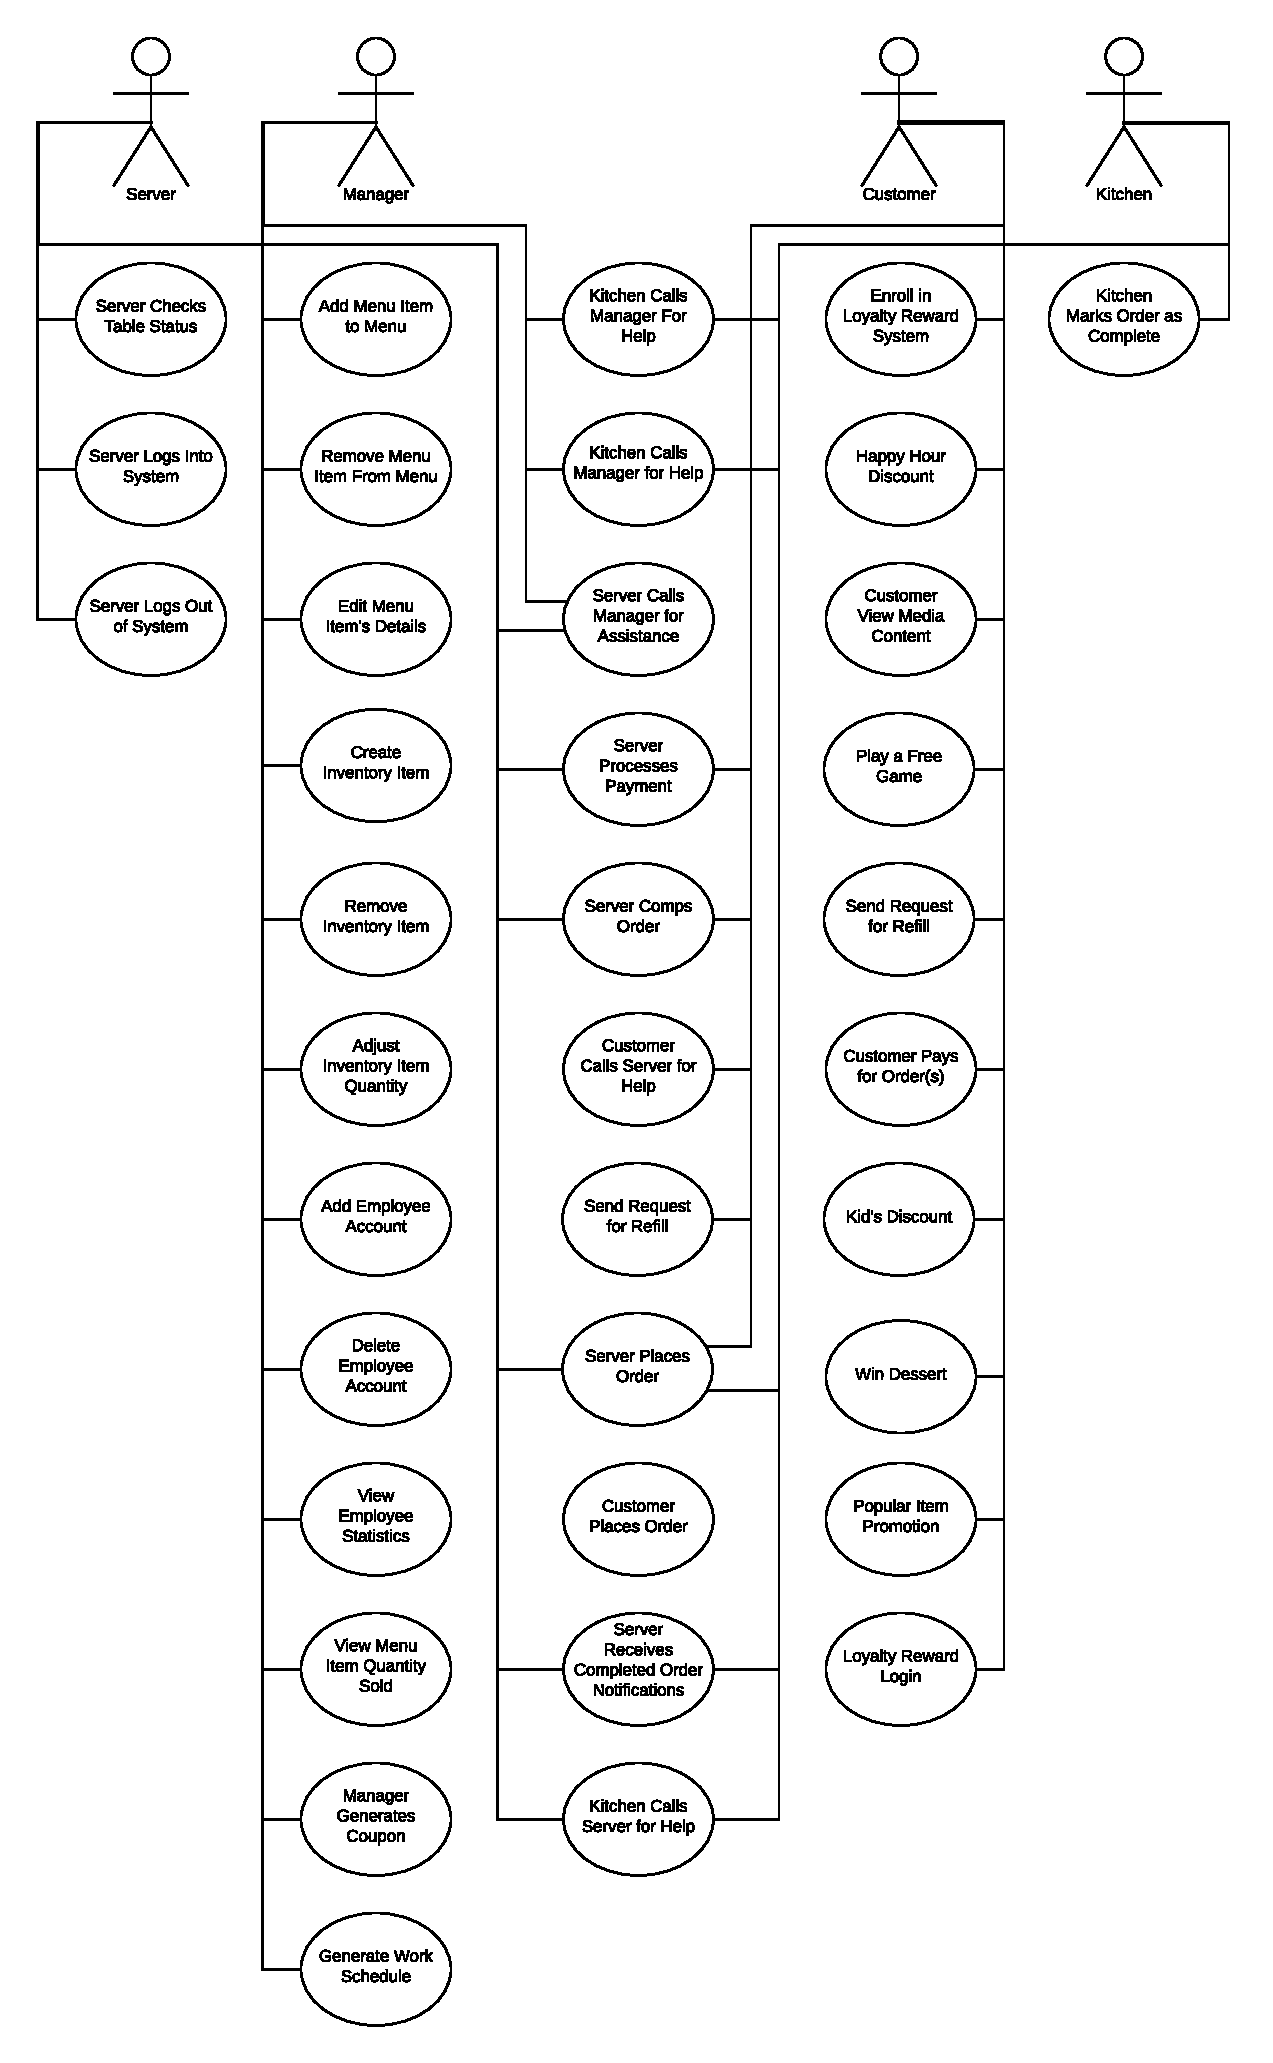
\includepdf[pages=-]{Part2/diagram.pdf}
\end{document}